% \documentclass[journal]{vgtc}                % final (journal style)
% \documentclass[review,journal]{vgtc}         % review (journal style)
% \documentclass[widereview]{vgtc}             % wide-spaced review
% \documentclass[preprint,journal]{vgtc}       % preprint (journal style)
% First we choose the document class (can be book, report, article etc.)
\documentclass[11pt]{article}
% \documentclass[11pt, twocolumn]{elsarticle}
% \documentclass{ieeetran}
\usepackage[margin=0.70in]{geometry} % Change Margins
\usepackage{mathtools}
\usepackage{textgreek}
\usepackage{graphics}
\usepackage[shortlabels]{enumitem} % Enum with letters
\usepackage{makecell}
\renewcommand\theadfont{\bfseries\sffamily}



\title{Title of my document}
% \date{2019-0}
\author{Flavio R. de A. F. Mello}

% Now we start the main document stuff
\begin{document}

\maketitle

\section{Domain and Task}

\section{Preprocessing}

    \subsection{File Format Normalization}
        A common issue when dealing with data science tasks is data formatting. Data is often stored in multiple different formats and schemas, regularly creating the need for normalizing the input before proceeding with the analysis. Computer vision is not free of such trappings. Considering just some of the more ostensibly used formats, there are at least 5 different image extensions (\textit{jpg, bmp, png, tiff, and gif}) and 5 video extensions (\textit{mp4, avi, mov, wmv, flv}). These numbers are increased when taking into account lesser known, and sometimes not open, formats. Considering different tools provide different level of support for each format, it is of interest to tackle this issue early on in the analysis pipeline, ensuring data flows seamlessly throughout the process. Luckily, given how pervasive this format plurality is, there is no shortage of tools available that can convert between the different file extensions.

    \subsubsection{Image Files Conversion}
        For the task at hand, there are 2 different image formats present in the data: \textit{jpg} and \textit{heic}. \textit{Jpg}, or \textit{jpeg}, is a longstanding open format with ample support in most ecosystems, while \textit{heic}, or \textit{heif}, is a newer format proposed as an alternative to \textit{jpg} being able to achieve higher compression. Most notably, it became the standard photo format on iOS 11. Given that the platform being used for the analysis (Matlab) provides support for \textit{jpg}, but not for \textit{heic}, it was decided to convert all the \textit{heic} files in the dataset provided into \textit{jpg}. This was done using the open source tool ImageMagick, which provides support for display and manipulation for multiple image formats. Additionally, the tool is available in all major ecosystems both desktop (Windows, OSX and Linux) and mobile (iOS and Android). Using windows, this can be done with a single line in the command prompt:

        \texttt{mogrify  -format jpg   *.heic}

        This command converts all \textit{heic} images found in the current path into \textit{jpg}, and outputs them in the same folder, while keeping the filename prefix the same.

    \subsubsection{Video Files Conversion}
        For this particular task, no video conversion was needed, the video formats encountered were \textit{.mp4} and \textit{.mov}, both fully supported by Matlab.

    \subsection{Video Frame Extraction}
        The face recognition techniques used in this study rely on static images only, therefore in order harness the benefits of having video data available, it was decided to extract individual frames from the video files, and include these frames in the pipeline along with the pictures provided in the dataset. This can be done rather efficiently in Matlab as it provides native support for reading individual frames from video content. When extracting frames, it was decided not to keep every single frame, as this would exponentially increase the number of images/faces to be labeled at further stages in the preprocessing pipeline - even though movies taken from individual people (and its resulting frames) are easily labeled, there is still the matter of group videos, where there is no easy way of labeling extracted faces without relying on manual input in some way - this is further discussed in section \ref{sec:face_labeling}. Considering this study is for didactic purposes, it was decided to keep only every 5th frame from the videos provided, as a way to balance the time spent in other stages of the facial recognition pipeline while still understanding of the difficulties involved in the data grooming necessary to have an effective pipeline. An additional complication in video frame extraction is that some of the provided videos have a fadeout effect which gradually decreases the image brightness to 0. Although having examples of the same person in different lighting and brightness levels may be favorable to training a model which is more robust against changes in lighting, this may be problematic because some of the frames are effectively too dark for human eye to distinguish the subject, although it is expected for the face extraction to ignore said frames since no faces would be found, in my initial tests, the face extraction step did recognize as faces some undesirable sections, thus requiring further manual input to remove these pitch black images from the labeled dataset. As an attempt to diminish this effect, when extracting video frames, a minimum brightness threshold is used to ignore images that are deemed as "too dark".
        It is important to note how the addition of video based data, enabled by the increased dissemination of portable electronics able to record high definition videos, is an important upgrade on static pictures based data only. Videos capture slight changes and nuances in the image which prove valuable when training an image based classifier. Considering that the effort, time and cost required to record a video is nearly the same as a picture, and that videos provide orders of magnitude more frames to be processed, it would be sensible to resort to video based data unless the increased definition provided by static pictures is required.

    \subsection{Face Extraction}
        Having already preprocessed all videos and labeled the individual content, the next step in the preprocessing pipeline is to extract individual faces from the entire content (i.e. both single and group images/frames). This can be done in multiple different ways and, in part, also depends on how the latter stages of the facial recognition pipelines are designed. For example, if the recognition techniques rely on a specific size or aspect ratio, it may be best to include these constraints when extracting/cropping the face regions instead of simply resizing images at a latter stage as, such resizing can introduce artifacts or distortions that may decrease the accuracy of the trained models - this is specially true for changes in the aspect ratio. In this study, the face extraction stage can be divided into three substages: face detection, face cropping, and data cleaning.

        \subsection{Face Detection}
            In order to extract faces from a natural image, one must first locate where the faces are localized. In this study, this was done using Matlab's pretrained 'FrontalFaceCART' Cascade Object Detector which relies on Haar features to locate faces within an image.

        \subsection{Face Cropping}
            Once each face region is detected they are then cropped, resulting in a new image containing only the face. The method of doing may depend on how latter stages of the pipeline are setup, as mentioned above. In this study, it was decided to work with square images of faces - based on University of Oxford's Visual Geometry Group approach, taken in VGG-Faces. That is, when cropping the facial regions, ensure the cropped region is a square one, and already resizing the resulting crop into the exact dimensions used to feed images to the CNN. Even though some of the feature types used for non-CNN classification techniques are scale independent (e.g. SURF), it was decided to include the resizing step in all faces for the sake of simplicity and keeping the preprocessing pipeline unified. Therefore, the resulting image of face cropping is a 227x227, 3 channel RGB image that was resized using bicubic interpolation, in order to conform with alexnet's requirements.

        \subsection{Data Cleaning}
            It is expected for the face extraction algorithm to present some false positives (i.e. regions that are not in fact faces). It is desirable then to remove these images from the labeled sets so as not to affect the classifiers performance - having sections of peoples clothes could artificially increase its performance as all pictures were taken in the same day, with people keeping the same clothes in all pictures; conversely, having sections of the background along with the labeled faces could decrease model's accuracies as pictures were taken in the same locations, making the same background features visible in pictures from different subjects. For the purposes of this study, cleaning is done by manually going over all extracted sections and selecting ones which are not in fact faces. Finally, this collection of non-faces is saved for further use - this will be discussed in section \ref{sec:non-faces}.

\subsection{Face Labeling}\label{sec:face_labeling}
    Even though techniques such as CNNs rely on unsupervised learning concepts to determine the features to be extracted, facial recognition ultimately relies on supervised learning to match features to labels - in this case, numbers assigned to every participant. In this implementation, such labeling is done at two different stages in the pipeline. The first one, done before starting the preprocessing steps of image format conversion, the individual pictures and movies were already separated into individual folders with names matching each one's assigned label. Although this was done manually, it was done somewhat efficiently in the dataset provided, as each individual's pictures were taken sequentially and, thus images' metadata such as filename and creation date can be used to easily sort images in a way such that all images from a given person are found in a contiguous group. The second labeling task refers to labeling faces extracted from images/videos of the whole group. These provide a much more difficult task since there is no immediate way of bundling faces. Considering that a) there are 69 different individuals (i.e. labels) b) their respective labels are assigned arbitrarily and c) the human short-term memory capacity is restricted to the magnitude of 7 different items; any fully manual strategy of sorting the pictures will surely take too long and consume valuable time and resources. If we are to consider the applications of this pipeline in similar problem sets with a larger amount of labels, the resources needed to manually label each individual face would increase exponentially. As an effort to diminish the time taken to label these faces, I took the semi-automation approach. That is, to combine automatic and manual techniques so that the manual portions are enhanced, and therefore sped up, by the automation. For this purpose, two separate automation approaches were taken: I) Classification and II) Clustering. Both strategies and their perceived gains and pitfalls are stated below in sections \ref{sec:face_labeling:classifier} and \ref{sec:face_labeling:clustering}.
    \subsubsection{Label Automation: Classifier}\label{sec:face_labeling:classifier}
        As stated above, we already have at our disposal a subset of the face images that can be easily labeled (the ones taken from individual pictures/videos). Therefore we can train a facial recognizer with this subset only, and use it to predict the labels for faces taken from group data. This classifier will still perform worse when compared to one trained with the full dataset, especially considering the group pictures are the ones which introduce much of the scaling problem (i.e. faces from people in the back of the group have considerably smaller resolutions than ones from people in the front plane. Individual pictures were all taken at similar distances and resolutions). However, it still can be used to augment the labeling process. As limited as human short-term memory is, the human brain still excels at image comparing tasks, that is: to tell if two or more images are from the same subject. By leveraging a facial recognition classifier at this stage of the preprocessing pipeline we have the double gain of making the process more efficient, as well as creating a loose benchmark to compare how the classifier performed when trained with individual pictures only versus when trained with the full dataset, thus being able to gauge the effect of introducing the group subset in the train data. Implementation-wise, the strategy chosen was an iterative one. That is, establish a minimum prediction confidence threshold and label only predictions made with confidence level above said threshold. The intuition is that, by running this cycle multiple times (training and labeling), trained models' accuracies increase as more labeled data is made available which, in turn, enables the next trained model to confidently label part of the remaining data.
        In practice, however, this approach was not successful. The model tested was a Random Forest of 700 trees trained with the 500 most relevant SURF features. Based on the individual pictures alone, the trained model was not able to accurately classify faces extracted from the group shots. Even when restricting to the classifications made with the highest confidence (30-50\%) the classifications were often wrong. Based on these results, I opted to abandon this approach.
    \subsubsection{Label Automation: Clustering}\label{sec:face_labeling:clustering}
        After the failure of the classifier labeling approach, I decided to follow a slightly less automated one: clustering. In this methodology, instead of trying to predict the label of each face individually, all the faces extracted from the group data (over 30 000) are clustered using K-Means and images are then exported to separate folders according to their cluster id. This method does not have the benefit of automated labeling in the sense that it still requires manual input in the form of assigning a label to each face by recognizing the face and moving the file into its respective label folder. However, by grouping like images in folders some presorting is effectively made. Now it is more probable that a series of images belonging to the same label are ordered next to each other, furthermore, each folder contains only a small subset of different labels - in this experiment it was not rare to have folders with images from a single label and most folders containing up to 5 different labels. This setup vastly improves the labeling speed, by traversing a list of like images, the human vision system is able to quickly identify if any outlier is present. This method relies, then, on having as many images from the same person in a row as possible so that the label discovering is done only once for a large group of images. Needless to say, the number of clusters used plays an important role in providing proper grouping. Smaller amount of clusters increases the likelihood of having individual clusters with multiple labels. Conversely, if the cluster number if too large, what would be a single large chunk can be separated into multiple clusters. For the purpose of this task, I opted to cluster the data into 100 clusters (approximately 1.5x the amount of labels) to provide some separation while keeping the number of folders manageable. I then proceeded to labeling the data iteratively by focusing on these larger chunks of images, and ignoring groups/folder which had too may different labels to enable a efficient form of selecting large groups. Figure \ref{fig:label:samples} shows a few examples of the data resulting from clustering.
        \begin{figure}[ht]
            \centering
            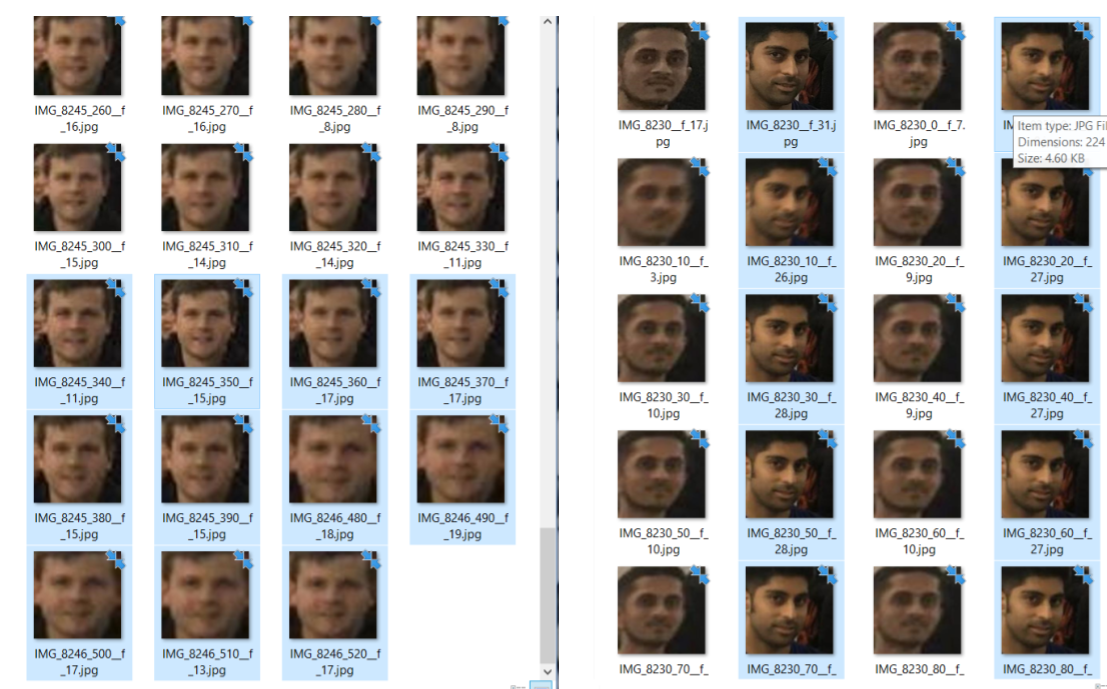
\includegraphics[height=4cm]{./Images/labeling/samples.png}
            \caption{Examples of image groupings resulting from clustering. Contiguous groups (left) are preferred, but some patterns allow for quick vertical selection as well (right)}
            \label{fig:label:samples}
        \end{figure}

        Once all the larger groups were labeled, I simply reclustered the remaining data into another 100 clusters, as the vast decrease in unlabeled data would naturally cause new clusters to be better grouped. Table \ref{table:cluster_passes} shows the amount of labeled images per clustering event. After only 3 epochs, the complete dataset of faces extracted from group pictures/movies was processed.

        \begin{table}[h!]
            \centering
            \begin{tabular}{||c c c||}
                \hline
                Cluster Epoch & Sorted Images & Acc. Sorted \% \\ [0.5ex]
                \hline\hline
                1 & 23527 &  65\% \\
                \hline
                2 & 7587 &  86\% \\
                \hline
                3 & 2410 & 92\% \\
                \hline
           \end{tabular}
           \caption{Group Image Labeling Through Clustering Progress}
            \label{table:cluster_passes}
        \end{table}

        For the improving the efficiency of label recognition, I set up a simple visual reference chart by selecting one sample image from each individual and naming them according to their respective labels. This provided a fast and important visual cue for remembering every single label. Figure \ref{fig:label:cheatsheet} shows this reference sheet.

        \begin{figure}[ht]
            \centering
            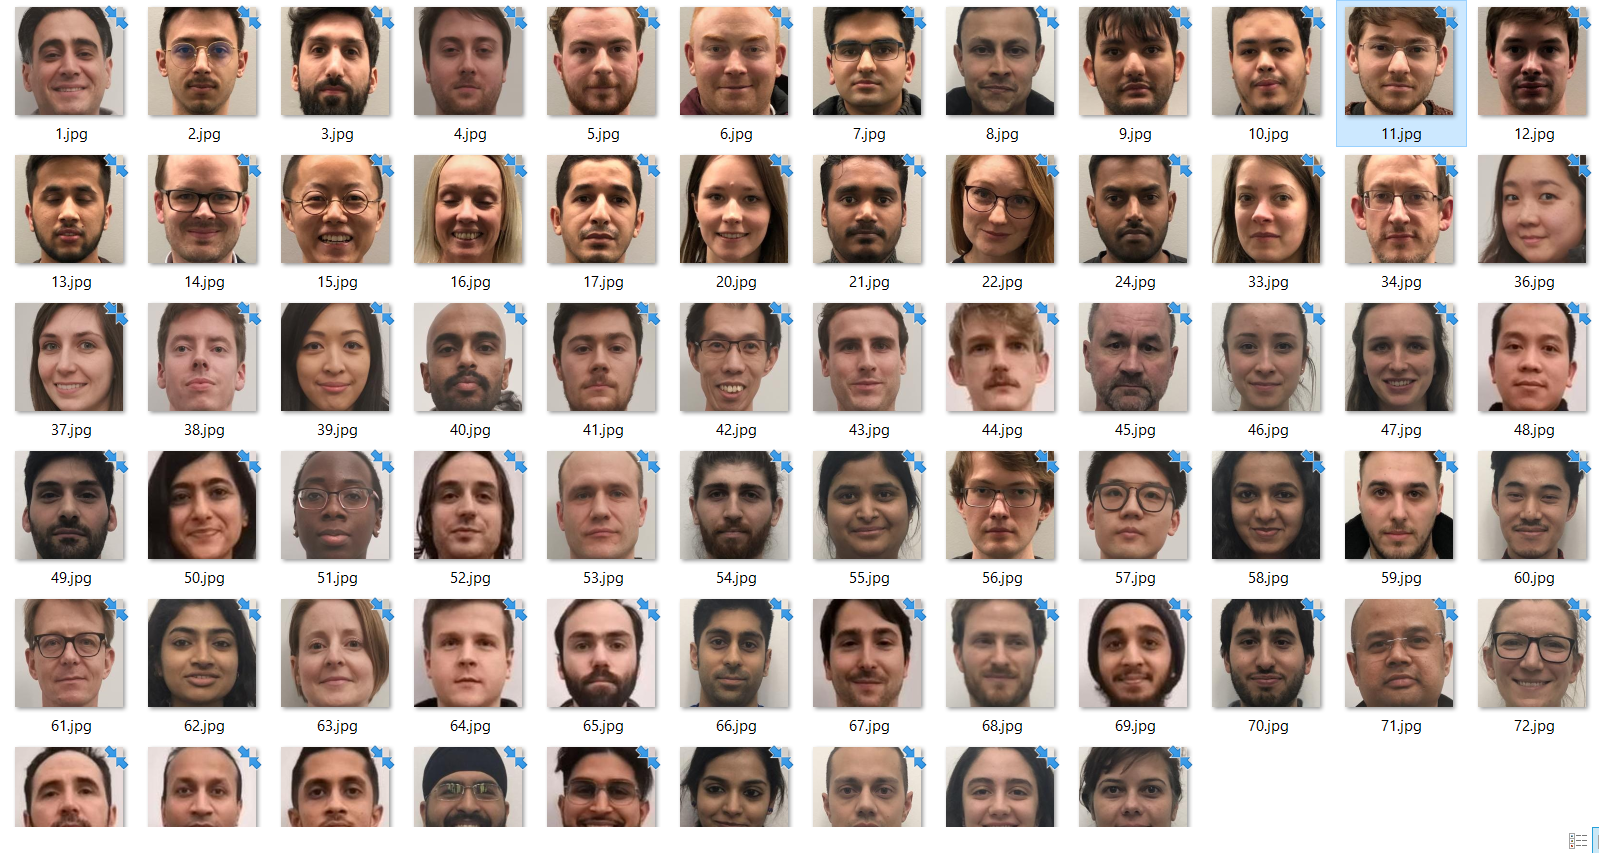
\includegraphics[height=4cm]{./Images/labeling/cheatsheet.png}
            \caption{Labeling Reference Sheet}
            \label{fig:label:cheatsheet}
        \end{figure}

    \subsubsection{Label Results: Outliers and Unlabeled}\label{sec:face_labeling:outliers}
        During the labeling process a few outliers were noted they are present in this section:

        \subsubsubsection*{Unlabeled Individuals}\label{sec:face_labeling:outliers:unlabeled}
            In the group data, there are some individuals who are not present in the labeled individual pictures. This could be either because they simply not present in the lab section when the labeling was made, or they chose not to be labeled. In this particular case, I opted to ignore these images and not include them in the dataset. Despite knowing the face extraction step will still select these faces when presented with a group image, and they will inevitably be classified as another individual - one of the properly labeled ones. This choice was made based on the fact the, prior to training the classifiers, the full dataset is trimmed to ensure all classes have the same amount of data to ensure there is no distribution bias in the models: That is that they classify based on the features alone, and not on some expected distribution of the classes. Each face has the same probability of appearing, and any discrepancies in the amount of data available is either due to minor changes in the human data collection (e.g. videos of not the exact same length) or, in other cases, or due to difficulties in the face detection algorithm used (further explained in section \ref{sec:face_labeling:outliers:difficulties}). If I was to include these faces as labels, the amount of data used for training would be vastly reduce given that these individuals have considerably less examples than the other ones. Figure \ref{fig:label:unlabeled_inds} shows the individuals in question.
            \begin{figure}[ht]
                \centering
                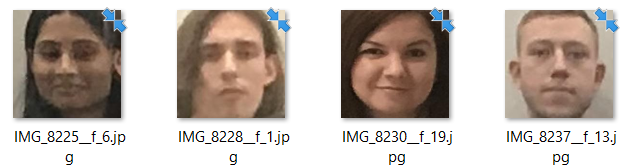
\includegraphics[height=4cm]{./Images/labeling/unlabeled_inds.png}
                \caption{Individuals that did not have individual pictures with labels}
                \label{fig:label:unlabeled_inds}
            \end{figure}

        \subsubsubsection*{Unlabelable Images}
            Considering the faces were also extracted from video material, which is of considerably lower resolution than the images, some of the faces were too unfocused/blurred for me to be able to confidently label them. As they are singnificantly small in number when compared to the rest of the data, I opted to remove them from the dataset instead of risking introducing erroneous data by human error. Figure \ref{fig:label:blurry} shows some examples of images that were left out of the final dataset.
            \begin{figure}[ht]
                \centering
                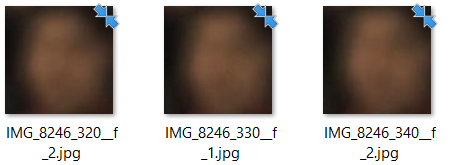
\includegraphics[height=4cm]{./Images/labeling/blurry.jpg}
                \caption{Images that were left out of the dataset due to extreme poor quality}
                \label{fig:label:blurry}
            \end{figure}

        \subsubsubsection*{Face Extraction Difficulties}\label{sec:face_labeling:outliers:difficulties}
            The face detection algorithm used leverages the Viola-Jones algorithm with Haar features to detect changes in shade in specific regions of the face, such as eyes, nose and forehead. It is known that this particular type of detection strategy is inherently biased (see http://gendershades.org/), being able to detect lighter skinned faces with considerably better than darker skinned ones. This effect was observed in more evidently in the faces extracted from the group data where one individual had around 20\% instances of her face detected when compared to the rest of the data. It is of the utmost importance to stress how this type seemingly innocent of bias could lead to unwanted biases in other critical applications of computer vision and should be combated, specially considering that face detection often lies at the initial stages of a computer vision based pipeline.


% \subsection{File Sorting}

\section{Facial Recognition}
    Once all the preprocessing and labelling is done, the actual image classification task is somewhat simple as there are powerful tools readily available for the task not only in Matlab, but also in other languages/stacks as well. This study focused on 2 visual feature extracting techniques - SURF and HOG - as well as 5 different classification methods - Convolutional Neural Networks (CNN), Naïve Bayes (NB), K-Nearest Neighbours (KNN), Support Vector Machines (SVM), and Random Forests (RF). The four latter methods are classical machine learning classification methods, which were adapted for image classification based on natural language processing techniques such as bag of words - treating the occurrence rate of each individual word in a document as a separate feature. For image classification, "visual" words are used, that is a collection of visual features is extracted from each image, and the occurrence rate of each feature (word) is the feature vector. Both SVMs and RFs then rely on using a graphical feature extracting technique (SURF or HOG in this case) to generate a feature vector based on the occurrence rate of said features in each image, and then feeding said feature vectors, along with their respective labels, to the classifier in order to train it. Predicting a label then requires the user to extract from the new image the occurrence rate of the same visual features, and feeding this into the classifier. CNNs, on the other hand, are different from classical machine learning approaches in that the neural network itself performs both the feature extracting and classification - this is further discussed in section \ref{CNN} below.

    \subsection{Histogram of Oriented Gradients - HOG}
        Histogram of Oriented Gradients is a somewhat simple feature descriptor that relies on sectioning an image in to a grid (with some overlap) and computing the orientation gradient for each of the local sections. When used for image classification, each section's gradient becomes a single feature, it requires then for all images to be of the same size so that the grid sections are comparable. It is, therefore, not particularly robust against changes in scale or orientation.
    \subsection{Speeded-Up Robust Features - SURF}
        Based on scale-invariant feature transform (SIFT), the Speeded-Up Robust Features (SURF) is another visual feature descriptor which is able to extract features in the form of image regions (i.e. blobs) that are invariant to scale and rotation. That is, a single feature represents the same visual blob at multiple different scales and rotations. This is achieved by applying filters of multiple different sizes. This is made possible because SURF relies on the use of integral images, which makes the computational cost of applying a filter constant, regardless of the size of the filter.
    \subsection{Support Vector Machine - SVM}
        Support Vector Machines are a family of machine learning algorithms often used in classification tasks. Even when resorting to a linear kernel, they are able to separate non linearly separable data by mapping the data to a higher dimensional space, one in which data may be linearly separable.
    \subsection{Random Forest - RF}
        Random forest is another instance of machine learning algorithm that can be used for classification or regression tasks. Its name derives from the fact a random forest relies on growing multiple decision trees based on the data provided. This is done with feature bagging (i.e. each tree is grown with a random subset of the features) to reduce the bias of the forest as a whole. Once all the trees are grown (i.e. the forest is model trained), prediction is done by traversing all trees with the new sample data, and voting between the trees resulting classification.
    \subsection{Naïve Bayes - NB}
        Naïve Bayes is a family of classifiers that rely on Bayesian inference. Prior probabilities are computed from the training data and used when prediction values for new observations. It presumes that the features are independent between themselves which is often not true in complex scenarios.
    \subsection{K-Nearest Neighbours - KNN}
        K-Nearest Neighbours is a simple yet powerful classification algorithm that predicts labels based on the euclidean distance from the new observation to the training data, assigning the label according to the majority of the K-Nearest datapoints found in the training data.

    \subsection{Convolutional Neural Network - CNN}\label{CNN}
        Convolutional Neural Networks are a newer class of learning algorithms based on deep neural networks. They are considered "end-to-end" visual learning algorithms in the sense that a single CNN provides both the feature extraction and machine learning (most often than not, classification) capabilities. Feature extraction is done by use of multiple convolutional and pooling layers which have the effect of consolidating increasingly large receptive fields into a smaller number of values. Furthermore, the exact filters applied in the convolutional steps are randomly initialized. It is through learning, made via the backpropagation algorithm, that the most effective filters - and, therefore, visual features - are gradually selected within the network. Given the the sheer computational power required to run the backpropagation algorithm through a deep neural network, CNNs were only made possible by the exponential increase in computational power that happened over the course of the last 2 decades. The advent of discrete graphical processing units (GPUs), which excel at highly parallelizable tasks, were also an important factor in making CNNs feasible.

    \subsection{Unrecognized Faces}\label{sec:non-faces}
        As exposed in section \ref{sec:face_labeling}, it is more than expected for the facial face detection algorithm to have some false positive rate. This is true at the prediction stage just as much as it is during the preprocessing portion of the pipeline. However, at the prediction stage it is not possible to leverage human input to ignore these regions. One solution for dealing with this problem is to collect all the false positives found in the training stage and treat them as belonging to a new label representing all instances of non-faces extracted from the provided data. Then, if a given face is predicted as belonging to this label, it is ignored when outputting the results of the RecognizeFace function. This was the strategy implemented in this study. An alternative, which was not pursued, could be to ensure the predictors output, along with the predicted label, a confidence score and establish a minimum threshold, ignoring any predictions with scores below said mark.

    \subsection{Training Process}
        \subsubsection{Data Partitioning}
            As mentioned in section \ref{sec:face_labeling:outliers:unlabeled}, there are some discrepancies in the amount of data available for each individual. To ensure no bias is introduced in terms of data distribution, I opted to trim the dataset, forcing all classes to equally distributed in the dataset used. After said trimming process, the resulting balanced data is split into train and test sets according to a 85/15 ratio while keeping both subsets balanced as well. In both the trimming and train/test split, data is selected randomly from each label pool to be a part of the new dataset by use of the \texttt{'randomized'} flag in the \texttt{splitEachLabel} function.

        \subsubsection{Conventional Classifiers}
            For the conventional classifiers used (NB, KNN, SVM and RF), the training process is broken down into 2 steps. Feature extraction and training. Feature extraction entails in using either feature descriptor (SURF or HOG) to transform the raw images into a bag of features, which is then ready to be fed into the classifiers along with the image labels.
        \subsubsubsection*{HOG}
            HOG features are extracted according to an user-defined cell size which is used to traverse the complete image (with some overlapping) and calculate the oriented gradients for each subsection of the image. The number of features generated when using HOG is, therefore, a function of a) the image size, b) the cell size and c) the overlapping size. It is important for classification tasks then to ensure the exact same values for these three parameters are the same for all observations (training, testing and new predictions). For this experiment HOG features were extracted using an 8x8 cell, images were all 227x227x3 (RGB channel) and overlapping was kept at 50\%.
        \subsubsubsection*{SURF}
            SURF features are different than HOG ones in the sense that the number of features present in an image is variable and depends on the image contents as well rather than only in metadata and hyperparameters. It is necessary then for some form of feature selection to ensure all observations have the same amount of features - this is done by way of a feature bag. The original SURF features are extracted from every single image in the training set, the weakest ones are dropped (20\% in this study) and the resulting visual features are then clustered, using K-Means, as a form of quantization. These N clusters then become the bag of features which is used to encode raw images into N features. In this experiment N was kept at the default value - 500. This generate bag of features must be saved for future use in order to be able to transform new observations in the form of raw images into the feature vectors used in the classifiers.
            One important point is that, in this particular experiment, I was not able to build the bag of features using the complete dataset due to resource limitations on my development machine. The bag creation process is memory intensive, when using the complete dataset, it easily depleted the available memory (16GB) and even used some disk space as swap memory. Even then, the command failed in Matlab due to out of memory errors. The solution then was to build the bag of words using a subset of the data (50\% selected randomly while keeping class balance, totaling 8085 images), and then encode the complete training data before feeding it into the classifiers. Given the restrictions imposed by the hardware, this was a sensible compromise: even though the bag was built with a subset of the data, the high sampling rate from the video material means that consecutive extracted faces are highly similar and, therefore their underlying visual features should be as well. Furthermore the full training/testing sets were subsequently used to train and evaluate the models.

    \subsection{Prediction Process}
        The prediction process is somewhat straightforward. Given an image, the program leverages the same functions used in the preprocessing pipeline to detect, crop and scale the faces, resulting in two arrays: One containing the 227x227x3 images of the extracted faces, and another containing the X and Y points indicating the centre of the facial respective facial regions detected. Centre is calculated as the centrepoint of the rectangular bounding box detected by the cascading face detector.
        Then the program determines which model should be used based on the \texttt{featureType} and \textttt{classifierName} variables provided by the user; loads said model; extracts the corresponding features from the faces array (if necessary) and proceeds to predict the labels using the selected model. Once the labels are predicted, a filtering step is applied to remove from the list faces that were predicted to belong to the \textit{non\_faces} artificial label. Finally, the response matrix is assembled to conform to the specified format. Note that, for the feature extraction step, it is necessary to reuse the same featureBag used for training the SURF-based classifiers and the same cell size used for the HOG-based ones.
    \subsection{Classifier Results}
        The results, shown in table \ref{table:results}, indicate some clear differences between the feature types and classifiers used. In terms of accuracy, the classifiers performed quite well with most classifiers staying in the 75\%-85\% accuracy range. The best classifier in terms of accuracy was the CNN with ~90\% correct predictions in the test set, but that came at the expense of a considerably longer training time, over 2.5 hours in total.
        \begin{table}[h!]
            \centering
            \begin{tabular}{||c c c c c c p{5cm}||}
                \hline
                    \thead{Feature \\ Type} & \thead{Classifier} & \thead{Training \\ Time (s)} & \thead{Prediction \\ Time (s)} & \thead{Test Set \\ Accuracy} & \thead{Model \\ Size (GB)} & \thead{Obs.} \\ [0.5ex]
                \hline\hline
                HOG & NB & 800 & 58 & 78\% & 3.6 & - \\
                \hline
                HOG & KNN & 71 & 340 & 87\% & 3.4 & 5 NN \\
                \hline
                HOG & SVM & 6030 & 394 & 88\% & 4.4 & Linear kernel \\
                \hline
                HOG & RF & 612 & 28 & 84\% & 4.2 & 100 Trees \\
                \hline
                SURF & NB & 87 & 525 & 65\% & 0.34 & - \\
                \hline
                SURF & KNN & 0.57 & 5 & 80\% & 0.033 & 5 NN \\
                \hline
                SURF & SVM & 61 & 9 & 75\% & 0.056 & Linear kernel \\
                \hline
                SURF & RF & 74 & 2 & 84\% & 0.68 & 100 Trees \\
                \hline
                CNN & CNN & 9194 & 10 & 90\% & 0.23 & Transfer Learning based on AlexNet \\
                \hline
            \end{tabular}
            \caption{Facial Recognition Results by Feature and Classifier Type}
            \label{table:results}
        \end{table}

        The CNN was trained using transfer learning from the pretrained AlexNet, a general purpose object categorization CNN trained with the ImageNet database to recognize over 1000 object categories. It is interesting to note how a CNN trained on a different domain (object instead of face classification) still fared remarkably well when applying simple transfer learning. If the CNN was to be trained from scratch, it would be reasonable to expect better performance given the features captured in the initial convolutions/pooling layers of the CNN would be more relevant to the task at hand. On the other hand, we could also expect the total training time to be orders of magnitude longer.
        Comparing HOG and SURF based classifiers, the SURF-based ones were one order of magnitude smaller in size and faster to train. The training time becomes less discrepant if we factor in the time necessary to build the feature bag (SURF only) extract the training features, as SURF required ????s while HOG required only ???s for this preprocessing task. Despite being more efficient, the SURF models were, in general, less accurate than the HOG-based ones. It is important to note, however, that one of SURF's most relevant improvements over HOG - being invariant to scale and rotation - has diminished effect in this specific problem set as all faces are in the general upright direction and the cropping+scaling done in preprocessing means that the faces all have similar sizes when being fed into the classifiers.
        Finally
\subsection{Tuning}
\subsection{Model Selection}
\section{Digit Recognition}
\subsection{Strategy}
\subsection{Results}
\section{Full Program}
\section{Conclusion}
\section{reflection}
\section{Further Work}
- TF/IDF
- rotation leveling
- Tuning Hyperparameters
- CNN from scratch
- SURF/HOG cell sizes & other hyperparams (n clusters in SURF)

\end{document}
